% !TEX TS-program = pdflatexmk
\documentclass[12pt]{article}

% Layout.
\usepackage[top=1in, bottom=0.75in, left=1in, right=1in, headheight=1in, headsep=6pt]{geometry}

% Fonts.
\usepackage{mathptmx}
\usepackage[scaled=0.86]{helvet}
\renewcommand{\emph}[1]{\textsf{\textbf{#1}}}

% Misc packages.
\usepackage{amsmath,amssymb,latexsym}
\usepackage{graphicx,hyperref}
\usepackage{array}
\usepackage{xcolor}
\usepackage{multicol}
\usepackage{tabularx,colortbl}
\usepackage{enumitem}

\usepackage{fancyhdr}
\pagestyle{fancy} 
\lhead{\large\sf\textbf{MATH 316: History of Math}}
\rhead{\large\sf\textbf{Worksheet (\S 1.1-1.2)}}

\begin{document}
From our text:\\

Mayan Numerals\\


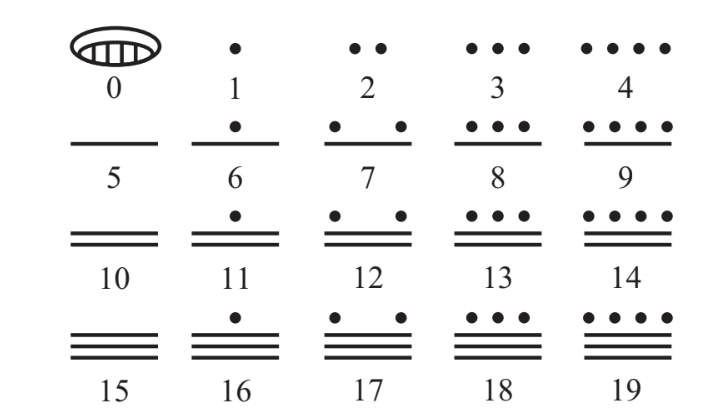
\includegraphics[scale=.6]{mayan}

\vfill

Egyptian Hieroglyphs\\

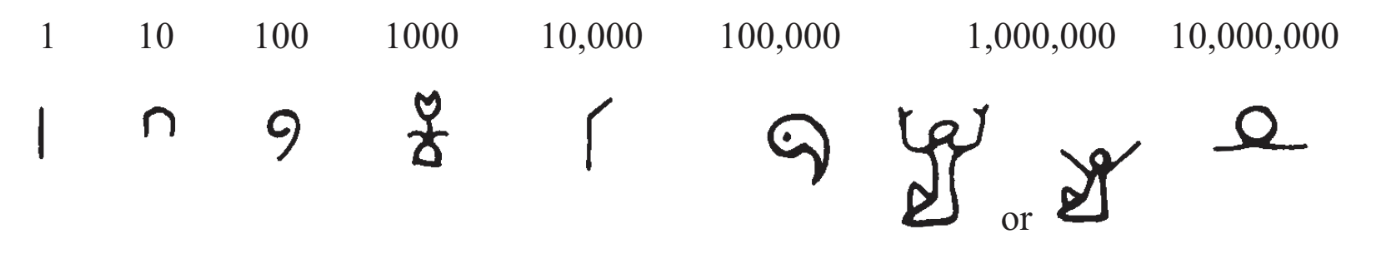
\includegraphics[scale=.6]{hieroglyphs}

\vfill

Ionian Alphabetic System\\

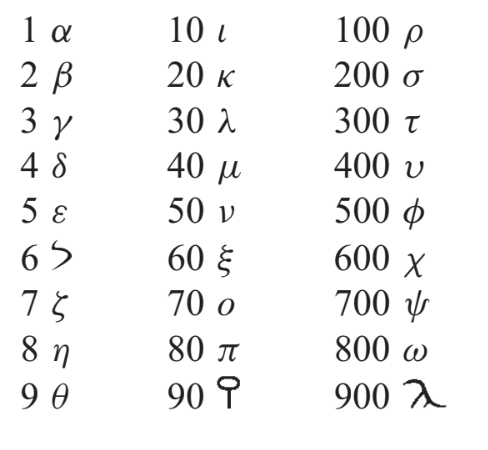
\includegraphics[scale=.7]{alphabetic}

\newpage
\begin{enumerate}
\item Write each number below in our system.
	\begin{enumerate}
	\item (Mayan)
	\vfill
	\item (Egyptian heiroglyphs)
	\vfill
	\item (Ionian alphabetic)
	\vfill
	\end{enumerate}
\item Write the number 9235 using each system below.
	\begin{enumerate}
	\item (Mayan)
	\vfill
	\item (Egyptian heiroglyphs)
	\vfill
	\item (Ionian alphabetic)
	\vfill
	\end{enumerate}
\newpage
\item Perform the operations below \emph{in the given numerical system}. Describe the algorithm and deduce the needed memorization.
	\begin{enumerate}
	\item (Egyptian)
	\vfill
	\item (Mayan)
	\vfill
	\item (Ionian alphabetic)
	\vfill
	\end{enumerate}
	
	

\end{enumerate}

\end{document}